%...existing code...
% !TeX root = main-report01.tex
\documentclass[12pt,twoside,a4paper,openany]{report}
% === Put them here, in the preamble ===

% Load project structure if available; don't fail LaTeX if file is missing
\input{../Structure4all.tex}

\input{headerfooter-report01.tex}

%------------------------%
%document DOCUMENT START
%------------------------%
\begin{document}

%cover
%
\includepdf[pages=-]{Cover (2)}
% Include substructure file if present; otherwise continue without error
\input{substructure-report01.tex}
\section{Abstract}
\input{abstract.tex}
\clearpage
\section{Introduction}
This is Our Team Intro.
\subsection{objectives}
This is objectives, such as what prof mention, Evaluate strength properties of wood (tension, compression, flexural strength) through lap joint testing
\subsection{Background}
This part we may describe about Brief theory on wood as an anisotropic material and importance of mechanical properties in timber design
\subsection{Standard References}
this part we may describe about Mention the testing standard used
\clearpage
\section{Materials and Methods}
\input{materialandmethod.tex}
\clearpage
\section{Results}
\input{result.tex}
\clearpage
\section{Calculations \& Analysis }
This is maybe the part that need all need to focus the most.

\clearpage
\section{Discussion}
\clearpage
\section{Conclusions}
%referennces
\phantomsection %Creates a hyperlink anchor (jump to that page when click)
\renewcommand{\chapter}{\section}
\renewcommand{\thechapter}{} % edit chapter numbering from here.
\renewcommand{\bibname}{References}  % change Bibliography -> References globally
%\thispagestyle{empty}  % optional: remove headers/footers
\begin{thebibliography}{99}
\addcontentsline{toc}{section}{References}
\bibitem{1} Let say it is References 1
\bibitem{2} Let say it is References 2 ...
\end{thebibliography}


% \clearpage

% \phantomsection %Creates a hyperlink anchor (jump to that page when click)
% \section*{Appendices}
% \markright{Appendices} % still make markright work eventhough using \section*{}
% \addcontentsline{toc}{section}{Appendices}
% This is appendices
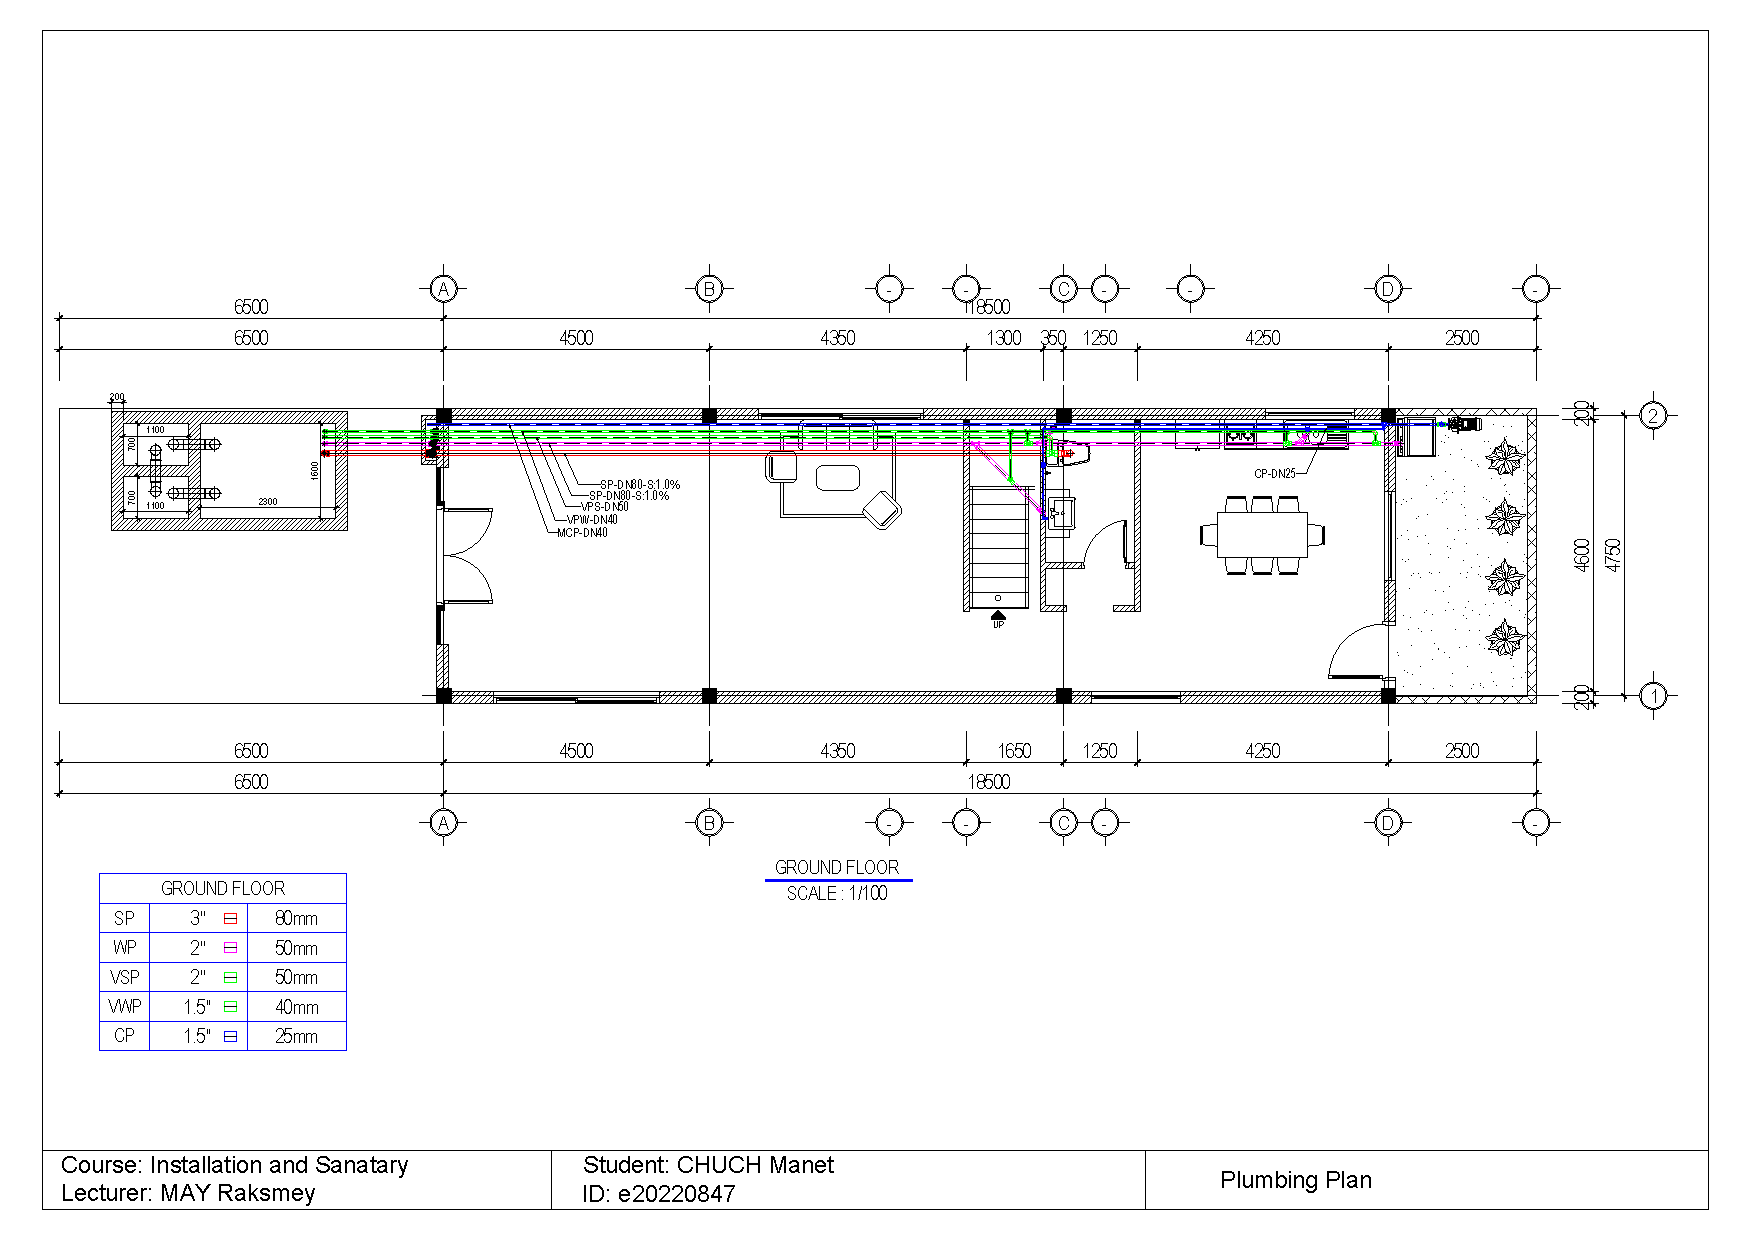
\includepdf[
    pages=-,
    scale=1,
    keepaspectratio,
    pagecommand ={\thispagestyle{maincontent}}
]{plan1.pdf}
This is  update of appendices
\end{document}
%...existing code...
